% !TEX program = tectonic
\documentclass[10pt,a4paper,landscape]{article}
\usepackage[margin=0.8cm]{geometry}
\usepackage[T1]{fontenc}
\usepackage[utf8]{inputenc}
\usepackage{lmodern}
\usepackage[french]{babel}
\usepackage{amsmath,amssymb}
\usepackage{xcolor}
\usepackage{booktabs}
\usepackage{tikz}
\usetikzlibrary{positioning,arrows.meta}
\definecolor{bleu}{RGB}{20,77,144}
\definecolor{vert}{RGB}{20,110,60}
\definecolor{orange}{RGB}{196,123,0}
\definecolor{rouge}{RGB}{160,30,30}
\definecolor{grisf}{RGB}{100,100,100}
\pagestyle{empty}
\setlength{\parindent}{0pt}
\begin{document}

% ══════════════════════════ PAGE 1 — LE FLUX ══════════════════════════
\begin{center}
{\LARGE\bfseries La stratégie adaptée --- la chronologie, étape par étape}\\[0.5mm]
{\small House uniquement (le Sénat n'a ni photos ni O/A/T : le mélanger fausserait tout) $\cdot$
notebook \textbf{indépendant} : inspiré du 05b, mais tout est redéfini et re-validé dedans}
\end{center}

\begin{center}
\begin{tikzpicture}[x=1cm, y=1cm,
  b/.style 2 args={rectangle, rounded corners=3pt, draw=#1, fill=#1!8, thick,
                   text width=#2, align=center, inner sep=6pt, font=\small},
  bl/.style 2 args={rectangle, rounded corners=3pt, draw=#1, fill=#1!8, thick,
                    text width=#2, align=left, inner sep=7pt, font=\small},
  fl/.style={-{Stealth[length=3mm]}, very thick, draw=grisf},
  lab/.style={font=\scriptsize\itshape, text=grisf, fill=white, inner sep=1pt}]

% ── É1-É2 : données et population ──
\node[b={grisf}{4.6cm}] (pop) at (4.0, 15.3)
  {\textbf{É2 --- la population}\\ \textbf{900} membres House\\ {\scriptsize passés par la Chambre, 2014--2026}};
\node[b={bleu}{6.2cm}] (traders) at (13.3, 15.3)
  {\textbf{305} tradent des actions cotées avec prix\\ {\scriptsize (107\,976 trades) --- les 595 autres ne tradent pas :\\ c'est pour ça que \og 900 \fg{} devient vite petit}};
\node[b={grisf}{4.9cm}, draw=grisf, dashed] (senat) at (22.6, 15.3)
  {{\scriptsize\textbf{É1 --- les 4 tables lues}\\ transactions PTR (clean) $\cdot$ photos d'entrée (15) $\cdot$ holdings (11) $\cdot$ trades O/A/T nets (16) --- sha vérifiés}};
\draw[fl] (pop) -- (traders);

% ── É3/É4 : les deux groupes ──
\node[bl={bleu}{11.6cm}] (gzero) at (6.6, 11.4)
  {\textbf{É3 --- G\_zéro : 185 membres SANS photo d'entrée} {\scriptsize(déjà en poste avant 2014, ou photo inexploitable)}\\[1.5mm]
   \textbf{rien ne change} : départ portefeuille vide, $h = 0$,\\[0.5mm]
   puis trade PTR après trade PTR :\quad
   achat : $h \mathrel{+}= \dfrac{\tilde v}{P(\tau(t))}$ \quad$\cdot$\quad vente : $h \mathrel{-}= \min(q, h)$};

\node[bl={vert}{12.6cm}] (gphoto) at (20.2, 11.4)
  {\textbf{É4 --- G\_photo : 120 membres AVEC photo d'entrée (H/C)}\\[1.5mm]
   \textbf{on part du portefeuille d'entrée}, au jour de son \textbf{dépôt} $f_0$ :\quad
   $h_0(m,i) = \dfrac{\tilde v_i}{P_i(\tau(f_0))}$\\[1mm]
   puis les trades PTR s'ajoutent \textbf{au fil de l'eau} (mêmes règles qu'à gauche)\\[0.5mm]
   {\scriptsize la vente d'une position héritée n'est plus tronquée ($h_0$ la couvre) $\cdot$ \textbf{zoom pas à pas : page 2}}};

\draw[fl] (traders.south) to[out=-90, in=90] node[lab, pos=0.45] {pas de photo} (gzero.north);
\draw[fl] (traders.south) to[out=-90, in=90] node[lab, pos=0.45] {photo d'entrée} (gphoto.north);

% ── É5 : O/A/T pour tous ──
\node[bl={orange}{25.4cm}] (oat) at (13.4, 7.6)
  {\textbf{É5 --- on ajoute les trades que seuls les rapports O/A/T contiennent --- pour TOUS les membres House} (chaque trade étiqueté \texttt{provenance = oat})\\[0.5mm]
   entonnoir tracé : $26\,115 \;\to\; -221$ \og exchange \fg{} $\;\to\; -14$ dates corrompues $\;\to\; -10\,319$ sans prix coté $\;\to\; -481$ doublons PTR (490 appariements) $\;=\; \textbf{14\,970}$ trades ajoutés
   {\scriptsize --- divulgués $\sim$374 j après ; même convention de date que les PTR (date de transaction)}};
\draw[fl] (gzero.south) -- (gzero.south |- oat.north);
\draw[fl] (gphoto.south) -- (gphoto.south |- oat.north);

% ── É6-É8 : moteur → stratégie → tableau ──
\node[b={grisf}{6.8cm}] (moteur) at (4.4, 4.3)
  {\textbf{É6 --- le moteur en parts}\\ {\scriptsize défini et validé DANS le notebook : parts $h$, valeur $\sum_i h_i P_i$, rendement time-weighted (parts de la veille) --- un apport ($h_0$) n'est jamais une performance}};
\node[b={grisf}{7.8cm}] (strat) at (13.4, 4.3)
  {\textbf{É7 --- la stratégie la plus simple}\\ {\scriptsize au 31/12 de chaque année : classement au \textbf{Sharpe} (éligible si $n_{\text{jours}} \ge 126$ et Sharpe $> 0{,}4$) $\to$ copier les $K^*$ meilleurs, poids $1/K^*$ (variante : inverse-vol), tenir un an --- $K^*$ \textbf{walk-forward} $\cdot$ \textbf{définitions : page 2}}};
\node[b={rouge}{8.6cm}] (tab) at (22.6, 4.3)
  {\textbf{É8 --- le tableau final : 4 runs House}\\ {\scriptsize A$_H$ témoin $\cdot$ B$_H$ $+$photos $\cdot$ C$_H$ $+$O/A/T $\cdot$ \textbf{D$_H$ $=$ les deux} --- $\times$ poids $\{1/K,\ \text{inv-vol}\}$ $+$ contrôle par groupe $\cdot$ \textbf{résultats : pages 4-6}}};
\draw[fl] (oat.south -| moteur.north) -- (moteur.north);
\draw[fl] (moteur) -- (strat);
\draw[fl] (strat) -- (tab);

% ── garde-fous ──
\node[b={grisf}{25.4cm}] (garde) at (13.4, 1.6)
  {\textbf{garde-fous} : la photo est injectée à sa date de \textbf{dépôt}, jamais avant (anti-triche) $\cdot$
   notebook indépendant : chaque brique re-validée dedans (recalcul à la main, 2\ieme{} méthode) $\cdot$
   chaque table montre son aperçu $\cdot$ \texttt{prices\_v2} jamais modifié};

\end{tikzpicture}
\end{center}

\newpage
% ══════════════════════════ PAGE 2 — LES ZOOMS ══════════════════════════
\begin{center}
{\Large\bfseries Les trois zooms --- tout ce qui se passe, pas à pas}
\end{center}
\vspace{-1mm}

\begin{center}
\begin{tikzpicture}[x=1cm, y=1cm,
  bl/.style 2 args={rectangle, rounded corners=3pt, draw=#1, fill=#1!8, thick,
                    text width=#2, align=left, inner sep=8pt, font=\small}]

% ── ZOOM 1 : le portefeuille d'un membre G_photo ──
\node[bl={vert}{25.8cm}] (z1) at (13.4, 13.2)
  {\textbf{ZOOM 1 --- construire le portefeuille d'un membre à photo (exemple bout en bout, un seul titre suivi : XYZ)}\\[1.2mm]
   \textcolor{vert}{\textbf{1 $\cdot$ 29/07/2021 --- sa photo d'entrée est déposée.}} Elle liste son patrimoine en fourchettes : \og ARAIX : \$15k--\$50k\fg{}, \og XYZ : \$50k--\$100k\fg{}\ldots\\
   chaque ligne $\to$ milieu $\tilde v = \tfrac{\underline v + \bar v}{2}$, converti en parts \textbf{au prix du jour du dépôt} :\quad
   $h_{\mathrm{XYZ}} = 75\,000 \div 150\,\$ = \textbf{500 parts}$\quad{\scriptsize(ARAIX : $32\,500 \div 59{,}47 = 546{,}5$ parts, etc.)}\\[1.2mm]
   \textcolor{bleu}{\textbf{2 $\cdot$ 10/03/2022 --- il déclare un achat PTR}} \og XYZ, \$15k--\$50k\fg{} :\quad
   $h_{\mathrm{XYZ}} \mathrel{+}= 32\,500 \div 160\,\$ = 203 \;\Rightarrow\; 703$ parts\\[1.2mm]
   \textcolor{rouge}{\textbf{3 $\cdot$ 15/09/2022 --- il déclare une vente PTR}} \og XYZ, \$100k--\$250k\fg{}, soit $q = 175\,000 \div 140\,\$ = 1\,250$ parts demandées :\quad
   $h_{\mathrm{XYZ}} \mathrel{-}= \min(1\,250,\,703) \;\Rightarrow\; 0$ part\quad{\scriptsize(sans la photo, le moteur n'aurait vendu que les 203 parts de l'achat --- c'est la troncature qu'on corrige)}\\[1.2mm]
   \textcolor{grisf}{\textbf{4 $\cdot$ chaque jour --- valeur et rendement.}}\quad
   $V(t) = \sum_i h_i(t{-}1)\,P_i(t)$,\qquad $r_m(t) = \dfrac{\sum_i h_i(t{-}1)\,P_i(t)}{\sum_i h_i(t{-}1)\,P_i(t{-}1)} - 1$,\qquad $\mathrm{NAV}_m(t) = \prod_{s \le t}\bigl(1 + r_m(s)\bigr)$\\[0.6mm]
   {\scriptsize pourquoi les \textbf{parts de la veille} $h(t{-}1)$ : le jour où la photo (ou un achat) entre, elle ne compte pas encore $\to$ \textbf{un apport n'est jamais une performance} (propriété testée numériquement dans le notebook) $\cdot$ rendements bornés à $\pm50\,\%$/j (anti-données corrompues)}};

% ── ZOOM 2 : la stratégie Sharpe, K walk-forward, 1/K ──
\node[bl={bleu}{25.8cm}] (z2) at (13.4, 6.9)
  {\textbf{ZOOM 2 --- la stratégie la plus simple : Sharpe $\cdot$ $K$ walk-forward $\cdot$ poids $1/K$}\\[1mm]
   à chaque coupe (dernier jour coté de l'année $Y$, $Y = 2015 \ldots 2025$), quatre gestes :\\[0.6mm]
   \textbf{1. noter} chaque membre sur son passé seulement : $\;\mathrm{Sharpe}_m(Y) = \dfrac{\overline{r_m}}{\sigma(r_m)}\sqrt{252}$ sur $r_m(s),\ s \le 31/12/Y$ --- éligible si $n_{\text{jours}} \ge 126$ \textbf{et} $\mathrm{Sharpe}_m > 0{,}4$ (la règle du 05b : le minimum de trades saute) ;\\[0.6mm]
   \textbf{2. choisir} $K$ \textbf{en marche avant} : $K^*(Y) = \arg\max_{K \in \{4,\ldots,20\}} \sum_{y \le Y} x_y(K)$, où $x_y(K)$ = l'excès annuel que le top-$K$ a réalisé l'année $y$ déjà jouée {\scriptsize(1\iere{} coupe sans historique : $K = 10$, milieu de grille)} ;\\[0.6mm]
   \textbf{3. copier} les $K^*$ meilleurs Sharpe en \textbf{parts} : $\mathrm{nbr}_k = \dfrac{w_k W}{\mathrm{NAV}_k(t_R)}$, tenir un an (buy-and-hold, autofinancé). Poids principal $w_k = 1/K^*$ ; \textbf{variante inverse-vol} $w_k \propto 1/\hat\sigma_k$ ($\hat\sigma_k$ estimée sur le passé $\le$ coupe) --- au 05b, l'inv-vol gagnait avec la sélection IR ($t\,0{,}94\!\to\!1{,}49$) mais faisait \emph{moins bien} que $1/K$ avec la sélection Sharpe : on tranche sur NOS runs ;\\[0.6mm]
   \textbf{4. évaluer} par années civiles : $x_Y = \prod_{t \in Y}(1{+}r_{\text{strat}}) - \prod_{t \in Y}(1{+}r_{\text{SPY}})$, \quad $t = \dfrac{\bar x}{\sigma(x)/\sqrt{n}}$ {\scriptsize($n = 11$ années $\Rightarrow$ seuil $t_{10} \approx 1{,}81$)}, \quad $\beta$ et $\alpha$ par régression $r_{\text{strat}} = \alpha + \beta\, r_{\text{SPY}} + \varepsilon$.};

\end{tikzpicture}
\end{center}

\newpage
\begin{center}
{\Large\bfseries Le tableau final, et la question du mélange des deux groupes}
\end{center}
\vspace{-1mm}

\begin{center}
\begin{tikzpicture}[x=1cm, y=1cm,
  bl/.style 2 args={rectangle, rounded corners=3pt, draw=#1, fill=#1!8, thick,
                    text width=#2, align=left, inner sep=8pt, font=\small}]

% ── ZOOM 3 : lire le tableau final ──
\node[bl={rouge}{25.8cm}] (z3) at (13.4, 13.6)
  {\textbf{ZOOM 3 --- lire le tableau final (chaque run = la même stratégie, seules les données changent)}\\[1.2mm]
   \textbf{A$_H$} --- PTR seuls, départ zéro : \emph{le témoin} --- que vaut la stratégie actuelle, House pur ?\\
   \textbf{B$_H$} --- PTR $+$ photos d'entrée : partir du patrimoine change-t-il les élus copiés et la perf ?\hfill B$_H$ $-$ A$_H$ $=$ \textbf{l'effet photo}\\
   \textbf{C$_H$} --- PTR $+$ trades O/A/T : les trades manquants changent-ils quelque chose ?\hfill C$_H$ $-$ A$_H$ $=$ \textbf{l'effet O/A/T}\\
   \textbf{D$_H$} --- PTR $+$ photos $+$ O/A/T : \textbf{la stratégie adaptée}, les deux corrections ensemble\hfill à comparer à A$_H$ et au seuil $t_{10} \approx 1{,}81$\\[1mm]
   chaque run est joué avec les \textbf{deux poids} ($1/K$ et inverse-vol) $\to$ 8 lignes $\cdot$ colonnes : excès/an vs SPY $\cdot$ $t$ $\cdot$ années gagnantes $\cdot$ $\beta$ $\cdot$ $\alpha$ ajusté\\[0.5mm]
   {\scriptsize verdict mécanique : si $t < 1{,}81$ partout, l'adaptation ne démontre pas d'alpha --- et B/C disent d'où vient le changement.}};

% ── ZOOM 4 : le mélange G_photo / G_zéro ──
\node[bl={orange}{25.8cm}] (z4) at (13.4, 7.6)
  {\textbf{ZOOM 4 --- le classement mélange G\_photo et G\_zéro : problème réel, réponse à trois étages}\\[1.2mm]
   \textbf{le problème} : le Sharpe des deux groupes n'est pas mesuré pareil --- G\_zéro $=$ NAV reconstruite depuis une petite base
   (bruit, ventes tronquées) ; G\_photo $=$ portefeuille complet dès le dépôt (NAV mécaniquement plus lisse, diversifiée).
   Le top-$K$ mixte peut donc préférer un groupe pour des raisons de \emph{mesure}, pas de talent.\\[0.8mm]
   \textbf{ce n'est pas une triche} : un copieur réel n'aurait exactement que cette information hétérogène --- mais il faut le \textbf{surveiller} :\\[0.8mm]
   \textbf{S1 $\cdot$ diagnostic} --- à chaque coupe : part de G\_photo dans les éligibles vs dans le top-$K^*$ (figure dédiée).
   Si le top-$K$ sur-représente nettement un groupe, le mélange pèse ;\\[0.6mm]
   \textbf{S2 $\cdot$ contrôle stratifié} --- la même stratégie jouée \textbf{dans chaque groupe séparément} (univers G\_photo seul,
   univers G\_zéro seul), pour A$_H$ et D$_H$ $\to$ 4 lignes de contrôle. Verdicts par strate $\approx$ verdict mixte $\Rightarrow$ mélange innocent ;
   sinon, on lit strate par strate ;\\[0.6mm]
   \textbf{S3 $\cdot$ en réserve} --- sélection à \textbf{quotas proportionnels} ($K \times$ part du groupe dans les éligibles),
   activée seulement si S1/S2 montrent un vrai déséquilibre --- pas par défaut : un quota est une contrainte de plus, pas une correction.};

% ── garde-fou de lecture ──
\node[bl={grisf}{25.8cm}] (z5) at (13.4, 2.6)
  {\textbf{ce qui a été corrigé sur remarque d'Alice} : éligibilité $=$ celle du 05b Partie II ($n_{\text{jours}} \ge 126$ et Sharpe $> 0{,}4$,
   sans minimum de trades) $\cdot$ pondérations $=$ $1/K$ principal $+$ inverse-vol en variante (les deux jouées partout)
   $\cdot$ le mélange des groupes est surveillé (S1) et contrôlé (S2) dans le même notebook, aucun run supplémentaire coûteux.};

\end{tikzpicture}
\end{center}

% ══════════════════════ PAGES 4-6 — CE QUI EN SORT ══════════════════════
\newpage
\begin{center}
{\Large\bfseries Ce qui en sort (1/3) --- les données, la population, le portefeuille d'entrée}\\[0.5mm]
{\scriptsize chaque chiffre sort d'une cellule exécutée du notebook (42 cellules, 0 erreur)}
\end{center}

\textbf{\textcolor{bleu}{É1 --- les données}}\quad
table clean : $134\,464$ PTR dont House $122\,814$ $\to$ fenêtre 2013-2026 : $122\,809$ ($315$ membres, $4\,340$ tickers) $\cdot$
photos d'entrée : $284$ déposées $\to$ $248$ membres exploitables ($9\,310$ lignes, $792$ M\$) $\cdot$
O/A/T sans écho PTR : $26\,115$ $\cdot$ map tickers $4\,653$ paires, $0$ conflit $\cdot$ $12$ fourchettes clean$\leftrightarrow$v1, écart $0$ $\cdot$
prix : $3\,927$ tickers chargés ($64$ corrompus exclus) $\to$ \textbf{$107\,976$ trades House avec prix}.

\vspace{2mm}
\noindent\begin{minipage}[t]{0.47\textwidth}\vspace{0pt}
\textbf{\textcolor{bleu}{É2 --- la population}}
\begin{itemize}
\item $900$ membres House $\to$ \textbf{305} tradent des actions cotées $\to$ \textbf{120} G\_photo / \textbf{185} G\_zéro (partition exacte : $120+185=305$ \checkmark) ;
\item les $595$ autres ne tradent pas d'actions cotées --- c'est pour ça que \og 900 \fg{} devient vite petit.
\end{itemize}
\vspace{2mm}
\textbf{\textcolor{vert}{É3/É4 --- le portefeuille d'entrée $h_0$}}
\begin{itemize}
\item \textbf{117 membres initialisables}, $6\,746$ lignes, \textbf{78,1\,\%} de la valeur des photos convertie en parts (le reste : fonds/OTC sans prix coté) ;
\item recalculé à la main : ARAIX $32\,500\,\$ \div 59{,}47\,\$ = 546{,}52$ parts \checkmark $\cdot$ AA $8\,000\,\$ \div 30{,}58\,\$ = 261{,}64$ parts \checkmark ;
\item valeur initialisée par membre : médiane \textbf{$741\,009$ \$}, max $78{,}3$ M\$ (G000599).
\end{itemize}
\end{minipage}\hfill
\begin{minipage}[t]{0.50\textwidth}\vspace{0pt}
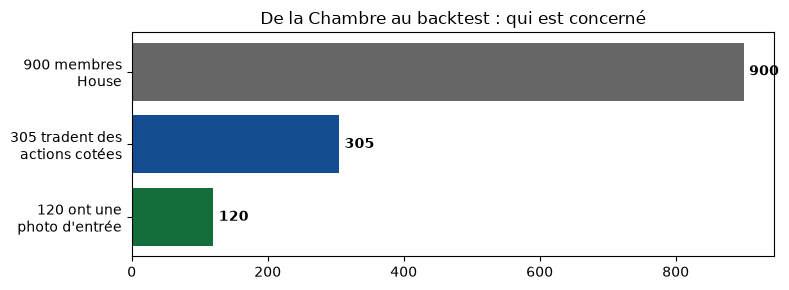
\includegraphics[width=\linewidth]{figures/fig_10_entonnoir.png}\\[1mm]

\includegraphics[width=\linewidth]{figures/fig_10_h0_couverture.png}
\end{minipage}

\newpage
\begin{center}
{\Large\bfseries Ce qui en sort (2/3) --- le flux unifié, le moteur, les 4 runs}
\end{center}

\noindent\begin{minipage}[t]{0.47\textwidth}\vspace{0pt}
\textbf{\textcolor{orange}{É5 --- les trades O/A/T, pour tous}}
\begin{itemize}
\item entonnoir : $26\,115 \to -221$ \og exchange \fg{} $\to -14$ dates hors fenêtre $\to 15\,451$ avec prix $\to -481$ doublons PTR ($490$ appariements) $=$ \textbf{$14\,970$ trades ajoutés} ;
\item flux unifié : \textbf{F $= 122\,946 = 107\,976$ ptr $+ 14\,970$ oat}, $424$ membres --- $119$ membres n'existaient QUE dans les rapports annuels ;
\item l'oat pèse le plus en 2023 : $1\,352$ achats oat contre $3\,573$ ptr.
\end{itemize}
\vspace{2mm}
\textbf{\textcolor{grisf}{É6 --- le moteur et les 4 runs}}
\begin{center}\small
\begin{tabular}{@{}lrr@{}}
\toprule
run & membres & tronqué \\
\midrule
A (témoin) & 226 & 937 M\$ \\
B ($+$photo) & 257 & 897 M\$ \\
C ($+$oat) & 362 & 1\,179 M\$ \\
\textbf{D (adaptée)} & \textbf{378} & 1\,122 M\$ \\
\bottomrule
\end{tabular}
\end{center}
\begin{itemize}
\item \textbf{(i)} fil rouge (G000599) refait en double boucle naïve : $869$ rendements identiques au moteur ;
\item \textbf{(ii)} photo seule $\Rightarrow r = 0$ exactement au jour de l'injection (2023-08-14) --- un apport n'est jamais une performance --- puis $-0{,}79\,\%$ le lendemain ;
\item \textbf{(iii)} B $\equiv$ A pour les membres sans photo.
\end{itemize}
\end{minipage}\hfill
\begin{minipage}[t]{0.50\textwidth}\vspace{0pt}

\includegraphics[width=\linewidth]{figures/fig_10_flux.png}\\[1mm]
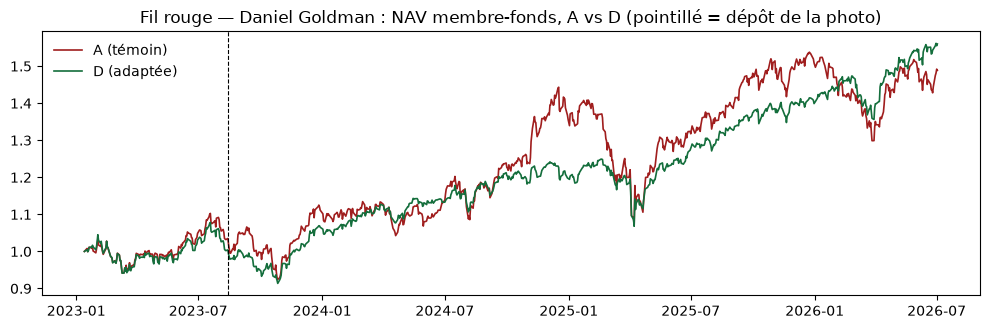
\includegraphics[width=\linewidth]{figures/fig_10_filrouge.png}\\[1mm]

\includegraphics[width=0.8\linewidth]{figures/fig_10_troncature.png}
\end{minipage}

\newpage
\begin{center}
{\Large\bfseries Ce qui en sort (3/3) --- la stratégie, le mélange, le verdict}
\end{center}

\noindent\begin{minipage}[t]{0.49\textwidth}\vspace{0pt}
\textbf{\textcolor{bleu}{É7 --- le tableau central}} {\scriptsize (11 années, seuil $t_{10} \approx 1{,}81$)}
\begin{center}\scriptsize
\begin{tabular}{@{}lrrlrrr@{}}
\toprule
run $\cdot$ poids & excès/an & $t$ & gagn. & $\beta$ & $\alpha$/an & $t_{\text{ap}}$ \\
\midrule
A $\cdot$ 1/K & $+0{,}9$ & $0{,}37$ & 4/11 & $0{,}99$ & $+0{,}6$ & $0{,}28$ \\
A $\cdot$ i-v & $-0{,}3$ & $-0{,}11$ & 4/11 & $1{,}00$ & $-0{,}5$ & $-0{,}27$ \\
\textbf{B $\cdot$ 1/K} & $\mathbf{+6{,}6}$ & $\mathbf{0{,}85}$ & 5/11 & $0{,}98$ & $+5{,}2$ & $\mathbf{1{,}55}$ \\
B $\cdot$ i-v & $+3{,}1$ & $0{,}60$ & 5/11 & $0{,}93$ & $+3{,}3$ & $1{,}33$ \\
C $\cdot$ 1/K & $-0{,}0$ & $-0{,}02$ & 4/11 & $0{,}92$ & $+0{,}9$ & $0{,}54$ \\
C $\cdot$ i-v & $-1{,}4$ & $-0{,}81$ & 5/11 & $0{,}83$ & $+0{,}9$ & $0{,}48$ \\
\textbf{D $\cdot$ 1/K} & $+0{,}9$ & $0{,}41$ & 4/11 & $0{,}90$ & $+1{,}9$ & $\mathbf{1{,}02}$ \\
D $\cdot$ i-v & $-0{,}2$ & $-0{,}11$ & 4/11 & $0{,}82$ & $+2{,}0$ & $1{,}00$ \\
\bottomrule
\end{tabular}
\end{center}
\begin{itemize}
\item \textbf{l'éligibilité change tout} : ancienne règle ($n_{\text{trades}} \ge 10$, run précédent) $\to$ témoin $-1{,}9\,\%$/an ($t\,{-}1{,}55$) ; règle du 05b $\to$ $+0{,}9\,\%$ ($t\,0{,}37$) ;
\item \textbf{inverse-vol perd contre 1/K sur toutes les lignes} (le constat du 05b Partie II se confirme) ;
\item meilleure ligne : \textbf{B $\cdot$ 1/K, $+6{,}6\,\%$/an} --- $t = 0{,}85$, 5/11 années : non significatif ;
\item éligibles : A $42 \to 184$ $\cdot$ D $50 \to 322$ ; $K^*$ : B verrouille $4$, D préfère $5$ ; oracle bloc 2018 recalculé à la main $\equiv$ moteur \checkmark ; sélection A vs D change à \textbf{11/11 coupes}.
\end{itemize}
\textbf{\textcolor{orange}{É7.2 --- S1/S2, le mélange}}
\begin{itemize}
\item \textbf{S1} : le top-$K$ sur-représente G\_photo certaines années --- 2020 : $80\,\%$ vs $26\,\%$ des éligibles $\cdot$ 2022 : $80\,\%$ vs $32\,\%$ --- et $0\,\%$ d'autres (2017, 2019, 2023, 2025) : le mélange pèse réellement ;
\item \textbf{S2} (chaque groupe séparément, 1/K) : A$\cdot$photo $t\,0{,}12$ $\cdot$ A$\cdot$zéro $-0{,}46$ $\cdot$ D$\cdot$photo $-0{,}11$ $\cdot$ \textbf{D$\cdot$zéro $0{,}80$ ($t_{\text{appr}}\,\mathbf{1{,}76}$)} --- aucun verdict de strate ne contredit le mixte ; les O/A/T aident surtout les \emph{sans}-photo.
\end{itemize}
\textbf{\textcolor{rouge}{É8 --- verdict}}
\begin{itemize}
\item aucune configuration ne franchit le seuil ($\max t = 0{,}85$ ; $\max t_{\text{appr}} = 1{,}76$ en strate) : \textbf{pas d'alpha démontrable}, robuste au poids, à la strate, au mélange ;
\item mais l'adaptée est \textbf{plus propre} ($\beta$ $0{,}99 \to 0{,}90$, $t_{\text{appr}}$ $+0{,}28 \to +1{,}02$) et l'effet photo (B) est la meilleure ligne ;
\item caveats : O/A/T datés à la transaction (divulgués $\sim$374 j après, notebook V1) $\cdot$ double comptage possible pré-dépôt $\cdot$ non-coté hors périmètre $\cdot$ \texttt{prices\_v2} intact.
\end{itemize}
\end{minipage}\hfill
\begin{minipage}[t]{0.48\textwidth}\vspace{0pt}

\includegraphics[width=\linewidth]{figures/fig_10_nav.png}\\[1mm]

\includegraphics[width=\linewidth]{figures/fig_10_s1.png}\\[1mm]
\begin{center}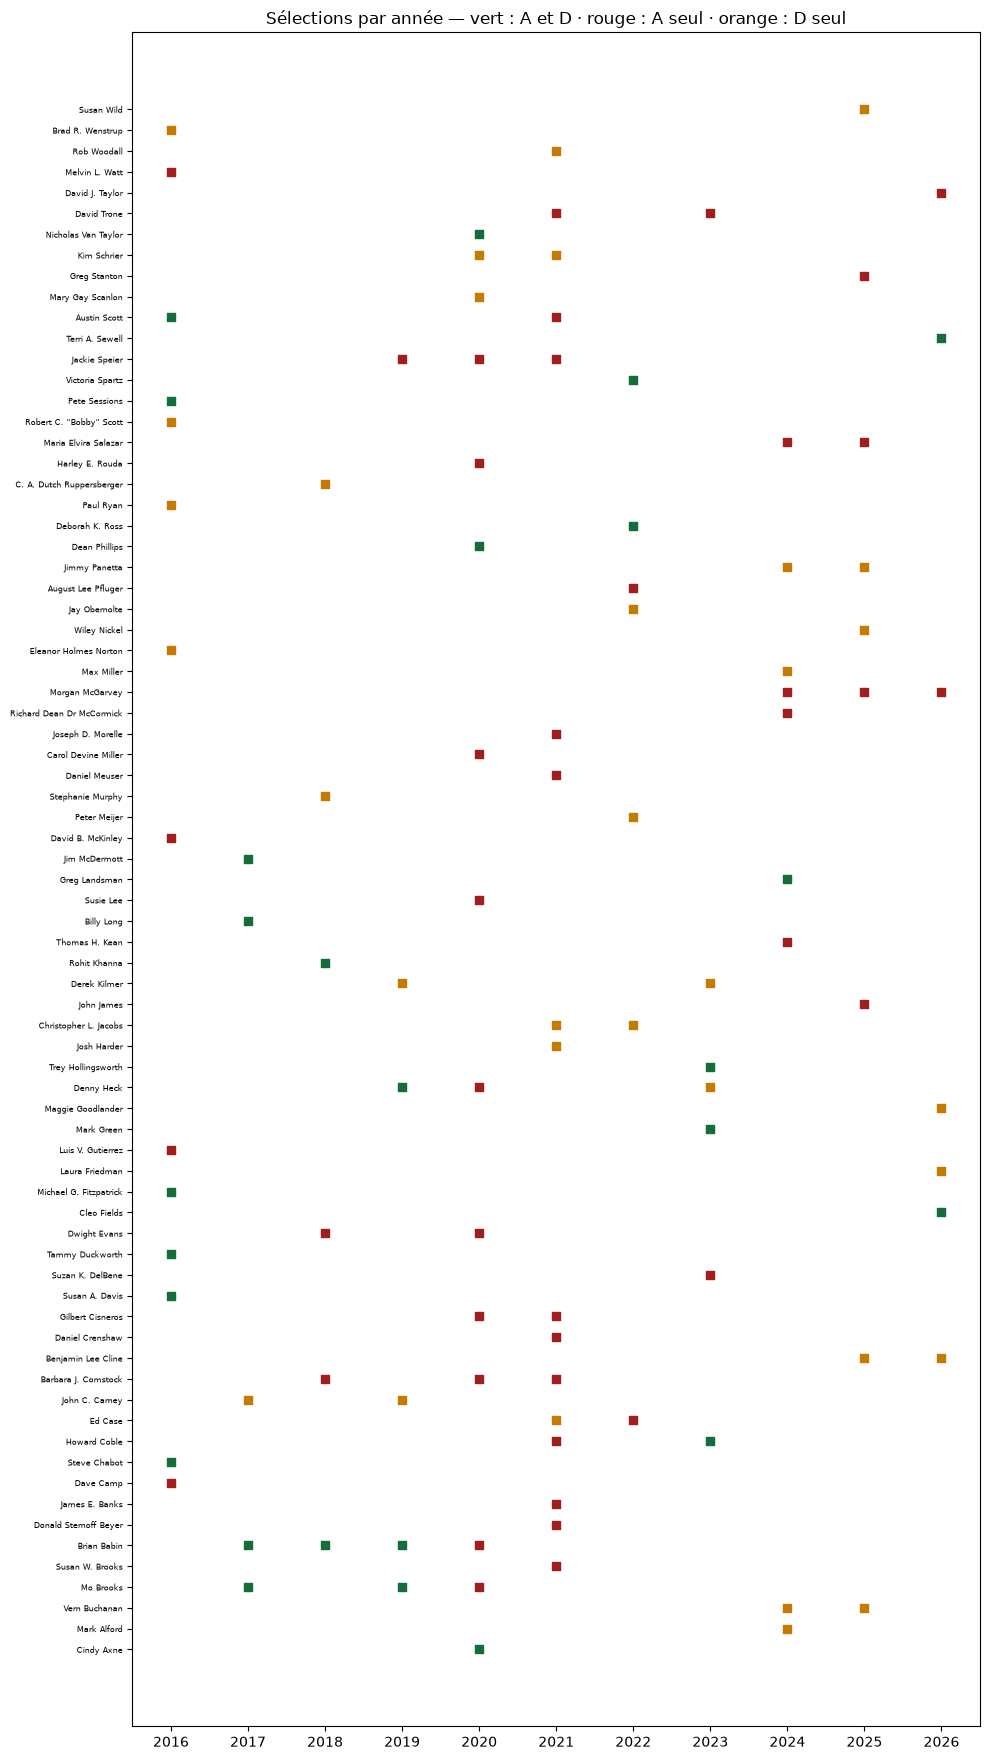
\includegraphics[width=0.85\linewidth,height=6.2cm,keepaspectratio]{figures/fig_10_composition.png}\end{center}
\end{minipage}

\end{document}

